\documentclass{article}

\usepackage{minted}
\usepackage[most]{tcolorbox}
\usepackage{geometry}
\usepackage{enumitem}
\usepackage{hyperref}
\usepackage{hyperref}
\usepackage[parfill]{parskip}
\usepackage{wrapfig}
\usepackage{accsupp}

\geometry{margin=0.8in}
\definecolor{lightgreen}{rgb}{0.56, 0.93, 0.56}
\definecolor{moonstoneblue}{rgb}{0.45, 0.66, 0.76}
\definecolor{magenta}{rgb}{0.8,0.66,0.76}
\begin{document}
\BeginAccSupp{}
\begin{flushright}
Computational Biology ~\\
Tufts University Bio 35 ~\\
Fall 2021 ~\\ ~\\
\end{flushright}
\begin{center}{\textbf{\Large{Spotlight 4: Rori Rohlfs}}}\end{center}

\textit{Please note that in general I have taken/adapted the words of our Spotlight subjects from their own websites to describe their work. I have done this in an effort to maintain accuracy in describing their research programs. Please do not copy paste text from their papers/websites in your assignments!}

\begin{wrapfigure}{L}{0.08\textwidth}
\begin{center}
 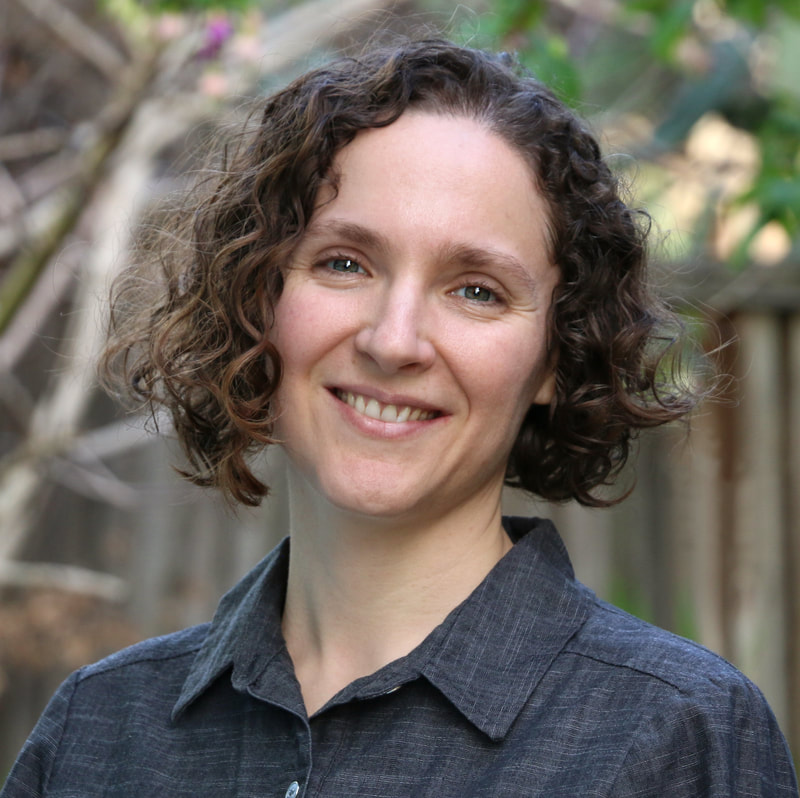
\includegraphics[width=0.09\textwidth]{images/rori-rohlfs.jpg}
 \end{center}
\end{wrapfigure}
~\\ As part of our unit on neutral evolution and population genetics, we are going to explore the work of Rori Rohlfs. Prof. Rohlfs' lab addresses questions about genetic variation within and between species. She applies and sometimes develops statistical methods to ask questions about variation in genetic sequences and RNA expression of those sequences. Dr. Rohlfs is a Professor at San Francisco State University.
~\\

Please read the following articles by Prof. Rohlfs: 
\begin{enumerate}
\item \texttt{\href{https://genestogenomes.org/understanding-our-eugenic-past-to-take-steps-towards-scientific-accountability/}{https://genestogenomes.org/understanding-our-eugenic-past-to...}}
\item \texttt{\href{https://www.genetics.org/content/211/2/363}{https://www.genetics.org/content/211/2/363}}
\end{enumerate}

Also watch the following short video:
\begin{enumerate}
\item \texttt{\href{https://www.youtube.com/watch?v=xpmlVuRPiRA}{https://www.youtube.com/watch?v=xpmlVuRPiRA}}
\end{enumerate}

\subsubsection*{Written Assignment} 
After reading Rori Rohlfs's articles and watching the video, write a reflection (max one page) on what you discovered. You might wish to address some of the following: 

\begin{enumerate}
\item What was most interesting to you in reviewing these resources?
\item What did you learn from these resources about the detection of relatives using genetic data, or the origins of population genetics as a field?
\item What new questions do you have after reviewing these resources?
\item What do these resources tell you about the types of people that do computational biology, or their motivations?
\end{enumerate}

\EndAccSupp{}
\end{document}
